%!TEX root = ../Main.tex

\chapter{Methodology}
The following chapter will describe the groups methodology and show multiple diagrams that show the behaviour of the system. These diagrams will be the following.

\begin{itemize}
	\item\textbf{Block Definition Diagram(BDD):} To provide an overview of the hardware structure.
	
	\item \textbf{Internal Block Diagram (IBD):} To provide an overview of the connection between IP-blocks.
	
	\item \textbf{Class Diagram:} To describe the logical partitions of the implemented software, and their dependencies and associations.
	
	\item \textbf{Activity Diagram:} To provide an overview of the overall system flow.
\end{itemize}

The block definition diagram show the overall context of the system and what the it consists of. 

\begin{figure}[H]
	\centering
	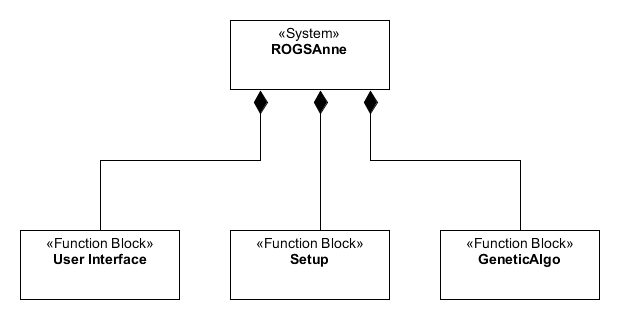
\includegraphics[width=\textwidth]{Images/BDD.png}
	\caption{Block definition diagram of ROGSAnne}
	\label{fig:BDD}
\end{figure}

The system consists of three function blocks. These blocks encapsulates some sort of functionality.

\begin{itemize}
	\item \textbf{User Interface} handles the interface between user and system. This is done through a console.
	\item \textbf{Setup} handles the initial creation of a population for the genetic algorithm. 
	\item \textbf{GeneticAlgo} will handle the optimization of the route with a genetic search algorithm.
\end{itemize}

An internat block diagram is made based on the BDD below. 

\begin{figure}[H]
	\centering
	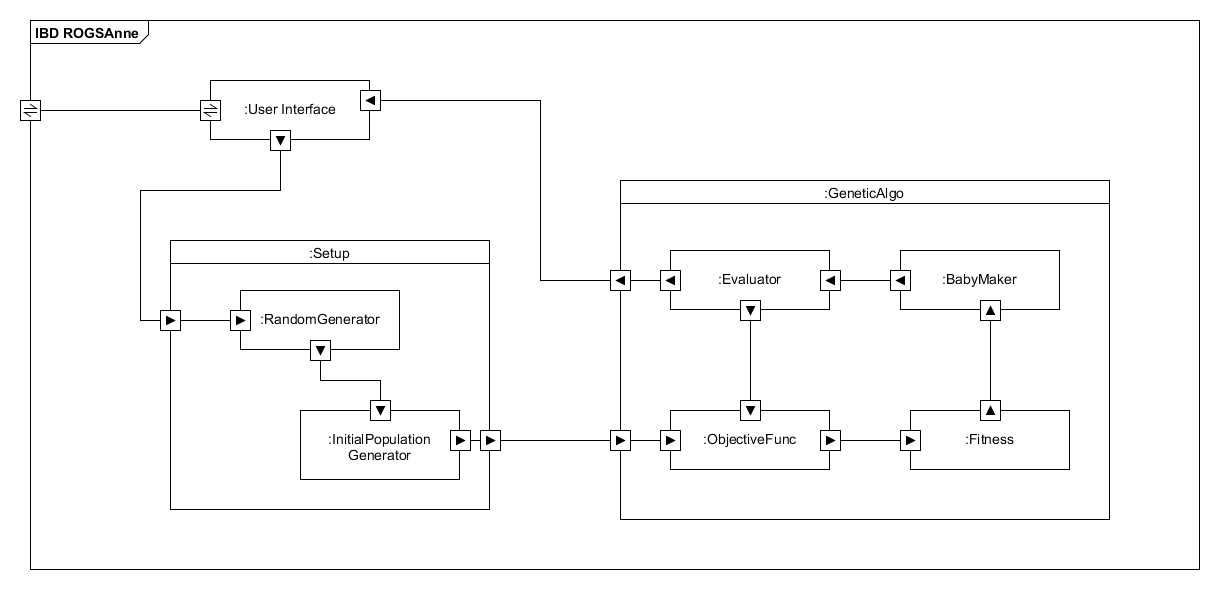
\includegraphics[width=\textwidth]{Images/IBD_ROGSAnne.png}
	\caption{Internal block definition diagram of ROGSAnne}
	\label{fig:IBD}
\end{figure}


